\chapter{A Ferramenta de Detecção}
A ferramenta para detecção de botnets foi desenvolvida utilizando o Ambiente de Desenvolvimento Integrado (\textit{Integrated Development Environment} - IDE) \textit{Qt Creator}. A tela inicial do sistema pode ser vista na Figura \ref{fig:initial_screen}.

\begin{figure}
\centering
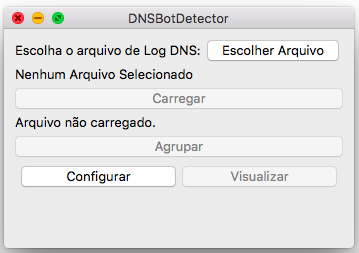
\includegraphics[width=10cm]{initial_screen}
\caption[Tela inicial da Ferramenta]{Tela inicial da Ferramenta} \label{fig:initial_screen}
\end{figure}

Qt é um IDE multi-plataforma que permite desenvolver aplicações com interface gráfica utilizando a linguagem C++ \citep{qtsite}. A escolha de Qt para o desenvolvimento da plataforma foi motivada pelo fato dele ser multi-plataforma, assim como o banco de dados utilizado (PostgreSQL), além do suporte à C++, que foi a linguagem adotada na fase inicial para implementar a preparação de dados.

A aplicação desenvolvida no Qt se comunica com o módulo desenvolvido em Python que serve de interface para leitura do banco de dados até o consumo final dos dados do banco, seja através de planilhas ou gráficos de distribuição espacial. As transações entre a interface gráfica e Python foram todas feitas através de criação de processos paralelos.

Ao longo dessa seção é exibida a documentação das funcionalidades do sistema, como o banco de dados foi modelado, além de uma visão geral sobre a aplicação desenvolvida.

\section{Documentação de Casos de Uso}
Nesta seção é mostrada a documentação dos casos de usos atendidos pelo sistema. São 5 casos de uso no total que podem ser vistos no diagrama de casos de usos exibido na Figura \ref{fig:diagram_use_cases}. 

\begin{figure}
\centering
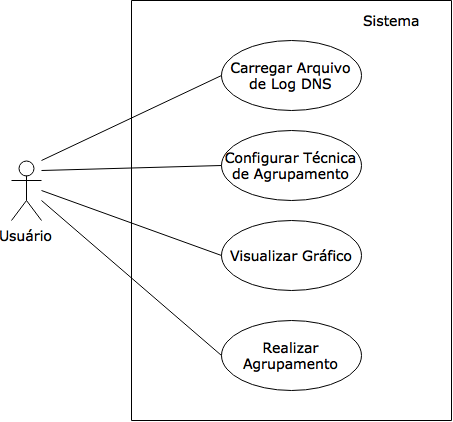
\includegraphics[width=12cm]{diagram_use_cases}
\caption[Diagrama de Casos de Uso]{Diagrama de Casos de Uso} \label{fig:diagram_use_cases}
\end{figure}

A descrição de cada caso de uso é feita em tabelas para melhor visualização. Essas descrições podem então ser vistas nas tabelas dessa seção. 

No modelo de especificação de casos de uso utilizado, os passos do Fluxo Básico de Eventos (FBE), são referenciados no Fluxo Alternativo de Eventos. Além disso, as pós-condições são atendidas quando o caso de uso é encerrado com sucesso. Nos casos de falha, a não ser que algo seja especificado, o sistema retorna ao estado em que estava antes do caso de uso ter sido iniciado.

O caso de uso Carregar Arquivo de Log DNS (Tabela \ref{tab:use_case_load_file}) é muito importante, já que concentra toda a lógica de tratamento de dados que será mostrada, em maiores detalhes, na seção \ref{sec:database_structure}. Nesse caso de uso, o usuário seleciona o arquivo que contém as informações brutas registradas pelo servidor de DNS para serem importadas na ferramenta. Nessa etapa de importação, os dados do arquivo são lidos e armazenados de uma forma estruturada em um banco de dados. Isso possibilita o cálculo das características de cada máquina que fez requisições ao servidor de DNS no período contido no arquivo.

\begin{table}[]
\centering
\caption{Caso de Uso - Carregar Arquivo de Log DNS}
\label{tab:use_case_load_file}
\begin{tabular}{|lp{10cm}|}
\hline
Nome: & Carregar Arquivo de Log DNS  \\ \hline
Ator: & Usuário   \\ \hline
Pré-condições: & Nenhuma   \\ \hline
\multirow{15}{*}{Fluxo Básico de Eventos:} & 1. O Usuário seleciona a opção ``Escolher Arquivo''  \\
 & 2. O Sistema exibe uma janela com os arquivos no formato txt presentes no sistema de arquivos do Usuário.  \\
 & 3. O Usuário seleciona um arquivo de log para importar.  \\
 & 4. O Sistema informa o endereço do arquivo selecionado e disponibiliza a opção ``Carregar''. \\
 & 5. O Usuário seleciona a opção ``Carregar'' \\
 & 6. O Sistema exibe um \textit{pop-up} informando que o arquivo está sendo importado para o banco de dados e inicializa a importação dos dados do arquivo para o banco de dados. \\
 & 7. O Sistema retira o \textit{pop-up} informando que o arquivo está sendo importado para o banco de dados e altera a mensagem ``Arquivo não carregado'' para ``Arquivo de Logs Carregado com Sucesso!'' e o caso de uso é encerrado com sucesso.\\ \hline
\multirow{3}{*}{Fluxo Alternativo de Eventos:} & \textbf{(A1) Nenhum Arquivo Selecionado:} No passo 4 do FBE se nenhum arquivo tiver sido selecionado.\\
 & A1.a) O caso de uso é encerrado com falha.\\ \hline
\multirow{5}{*}{Pós-Condições:} & 1. Os dados contidos no log informado pelo usuário foram carregados no banco de dados. \\
 & 2. As opções ``Agrupar'' e ``Visualizar'' são disponibilizadas.\\
 & 3. A opção ``Carregar'' é desativada.\\
\hline 
\end{tabular}
\end{table}

O caso de uso Configurar Técnica de Agrupamento, descrito na Tabela \ref{tab:use_case_config}, permite que o usuário selecione qual algortimo de agrupamento deseja utilizar e o número de grupos alvo. Além disso, pode selecionar quais características deseja que o algoritmo de agrupamento selecionado utilize. As preferências são persistidas em um arquivo no formado JSON, sendo utilizadas como padrão na próxima vez que a ferramenta for executada.

\begin{table}[]
\centering
\caption{Caso de Uso - Configurar Técnica de Agrupamento}
\label{tab:use_case_config}
\begin{tabular}{|lp{10cm}|}
\hline
Nome: & Configurar Técnica de Agrupamento  \\ \hline
Ator: & Usuário   \\ \hline
Pré-condições: & Nenhuma   \\ \hline
\multirow{12}{*}{Fluxo Básico de Eventos:} & 1. O Usuário seleciona a opção ``Configurar''  \\
 & 2. O Sistema recupera as informações do último arquivo de configuração salvo. \\
 & 3. O Sistema exibe as opções disponíveis para as Informações de Configuração, pré-selecionando as opções recuperadas no passo 2. \\
 & 4. O Usuário seleciona as Informações de Configuração desejadas.  \\
 & 5. O Sistema exclui o arquivo de configuração anterior, salva as Informações de Configuração selecionadas pelo Usuário em um novo arquivo de configuração e o caso de uso é encerrado com sucesso. \\
 \hline
\multirow{9}{*}{Fluxo Alternativo de Eventos:} & \textbf{(A1) Arquivo de Configuração Não Encontrado:} No passo 2 do FBE se o Sistema detectar que o arquivo de configuração anterior não existe.\\
 & A1.a) O Sistema utiliza os valores padrões como informação recuperada do arquivo.\\
 & A1.b) O Sistema retorna ao passo 3 do FBE. \\ 
 & \textbf{(A2) Janela de Configuração Cancelada:} No passo 5 do FBE se o Usuário cancelar a janela de configuração. \\
 & A2.a) O caso de uso é encerrado com falha. \\
 \hline
\multirow{2}{*}{Pós-Condições:} & 1. As Informações de Configuração selecionadas pelo Usuário são armazenadas no arquivo de configuração. \\
\hline
\multirow{10}{*}{Outras Informações:} & 1. Informações de Configuração: Lista de Características para Agrupamento, Algoritmo de Agrupamento e Número de Grupos. \\
 & 2. Valores Padrão: Lista de Características para Agrupamento: [\textit{count\_domain\_with\_numbers, average\_domain\_length, std\_domain\_length, count\_request, average\_requisition\_degree, std\_requisition\_degree, minimum\_requisition\_degree}], Algoritmo de Agrupamento: K-Médias, Número de Grupos: 4. \\
\hline 
\end{tabular}
\end{table}

Após realizar a carga do arquivo do log no banco de dados, o caso de uso Realizar Agrupamento (Tabela \ref{tab:use_case_clustering}) fica disponível. Nesse caso de uso, toda lógica de inteligência artificial é aplicada. Ou seja, o algoritmo de agrupamento é executado para a base de dados importada, utilizando as configurações presentes no arquivo de configuração no formato JSON. Os resultados, quais máquinas estão em cada grupo e as características não normalizadas de cada máquina, são armazenados em um arquivo no formato XLS e disponibilizados ao usuário.

\begin{table}[]
\centering
\caption{Caso de Uso - Realizar Agrupamento}
\label{tab:use_case_clustering}
\begin{tabular}{|lp{10cm}|}
\hline
Nome: & Realizar Agrupamento  \\ \hline
Ator: & Usuário   \\ \hline
\multirow{2}{*}{Pré-Condições:} & Os dados contidos no log DNS foram carregados no banco de dados.  \\ \hline
\multirow{13}{*}{Fluxo Básico de Eventos:} & 1. O Usuário seleciona a opção ``Agrupar''  \\
 & 2. O Sistema apresenta um ambiente para a escolha do destino do arquivo. \\
 & 3. O Usuário escolhe a pasta onde será salvo e o nome do arquivo. \\
 & 4. O Sistema agrupa os IPs segundo suas características resgatadas no banco de dados e aplica um algoritmo de agrupamento com parâmetros definidos no arquivo de configuração.  \\
 & 5. O Sistema salva os IPs e suas características na pasta escolhida pelo usuário. \\
 & 6. O Sistema exibe um alerta de que o relatório foi gerado e o caso de uso termina com sucesso. \\
 \hline
\multirow{3}{*}{Pós-Condições:} & 1. O arquivo no formato XLS é armazenado no endereço definido pelo Usuário com as informações de cada grupo separadas por aba. \\
\hline
\end{tabular}
\end{table}

Por fim, os casos de uso Visualizar Gráfico (Tabela \ref{tab:use_case_visualize}) e Identificar Cliente no Gráfico (Tabela \ref{tab:use_case_identify}) auxiliam no processo de investigação e seleção de características. Permitindo que o usuário visualize como as máquinas ficam distribuídas graficamente de acordo com as características selecionadas, além de permitir identificar qual é a máquina correspondente a um ponto especifíco no gráfico.

\begin{table}[]
\centering
\caption{Caso de Uso - Visualizar Gráfico}
\label{tab:use_case_visualize}
\begin{tabular}{|lp{10cm}|}
\hline
Nome: & Visualizar Gráfico  \\ \hline
Ator: & Usuário   \\ \hline
\multirow{2}{*}{Pré-Condições:} & Os dados contidos no log DNS foram carregados no banco de dados.  \\ \hline
\multirow{10}{*}{Fluxo Básico de Eventos:} & 1. O Usuário seleciona a opção ``Visualizar''  \\
 & 2. O Sistema exibe a Lista de Características para Agrupamento disponíveis para serem visualizadas. \\
 & 3. O Usuário seleciona 2 ou 3 características que deseja visualizar em um gráfico e seleciona a opção ``cria gráfico''. \\
 & 4. O Sistema buscará no banco de dados pelos endereços IP e as características selecionadas e apresenta os pontos resultantes em um gráfico e o caso de uso termina com sucesso  \\
 \hline
\multirow{5}{*}{Fluxo Alternativo de Eventos:} & \textbf{(A1) Quantidade de características inválida:} No passo 3 do FBE se o cliente selecionar qualquer quantidade abaixo de 2 e acima de 3.\\
 & A1.a) O Sistema exibe uma mensagem de erro e o caso de uso termina com falha.\\
 \hline
\multirow{2}{*}{Pós-Condições:} & 1. O Sistema exibiu o gráfico interativo com os eixos informados pelo Usuário. \\
\hline
\multirow{5}{*}{Outras Informações:} & 1. Lista de Características para Agrupamento: [\textit{count\_domain\_with\_numbers, average\_domain\_length, std\_domain\_length, count\_request, average\_requisition\_degree, std\_requisition\_degree, minimum\_requisition\_degree}].  \\
\hline 
\end{tabular}
\end{table}

\begin{table}[]
\centering
\caption{Caso de Uso - Identificar Cliente no Gráfico}
\label{tab:use_case_identify}
\begin{tabular}{|lp{10cm}|}
\hline
Nome: & Identificar Cliente no Gráfico  \\ \hline
Ator: & Usuário   \\ \hline
\multirow{2}{*}{Pré-Condições:} & O Sistema exibiu o gráfico interativo com os eixos informados pelo Usuário.  \\ \hline
\multirow{6}{*}{Fluxo Básico de Eventos:} & 1. O Usuário seleciona o ponto no gráfico que deseja identificar.  \\
 & 2. O Sistema recupera as informações do ponto, exibe em um rótulo no gráfico interativo o endereço de IP da máquina cliente no ponto desejado e o caso de uso termina com sucesso. \\
 \hline
 \multirow{2}{*}{Pós-Condições:} & 1. O Sistema exibiu o endereço de IP da máquina que estava no ponto selecionado. \\
 \hline
\end{tabular}
\end{table}

\section{A Estrutura do Banco de Dados} \label{sec:database_structure}
A leitura e identificação de cada campo do log individualmente não é o suficiente para representar as características que serão utilizadas pelos algoritmos de aprendizado de máquina. Ou seja, elas ainda precisam ser submetidas a diversos cálculos e tratamentos. Com o objetivo de acelerar o processamento desses tratamentos, além de facilitar e agilizar a consulta de informações posteriormente para efetuar uma investigação inicial dos suspeitos levantados pelo sistema, decidimos armazenar as informações em um banco de dados relacional.

O Sistema Gerenciador de Banco de Dados utilizado foi o PostgreSQL, como parte da nossa solução, para facilitar a escrita, leitura e atualização das informações coletadas dos registros DNS. Na modelagem feita, utilizou-se três tabelas para representar as informações contidas no log. A Figura \ref{fig:relational_diagram} apresenta a representação relacional do banco de dados, no qual já está incluso as características a serem analisadas como será esclarecido na seção \ref{sec:levantamento_das_caracteristicas}. Dessas três tabelas, a mais importante é a \textit{clients}, pois essa é a que realmente será utilizada pelos algoritmos de aprendizado de máquina. As tabelas \textit{dns\_queries} e \textit{domains} tem função apenas de auxiliar o cálculo da tabela \textit{clients}, porém podem servir também para consultas, caso alguém deseje utilizar a base de dados construídas para inspeção manual posterior.

\begin{figure}
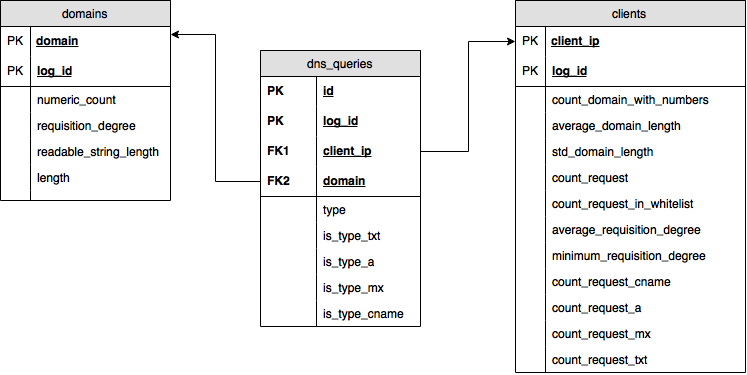
\includegraphics[width=\textwidth]{relational_diagram}
\caption[Diagrama Relacional do Sistema]{Diagrama Relacional do Sistema} \label{fig:relational_diagram}
\end{figure}

A tabela \textit{dns\_queries} é a que melhor representa a estrutura bruta do log de DNS. Mesmo sendo simples, sem muitos tratamentos, ela já apresenta consultas interessantes, como verificar que domínios uma máquina consultou. Os campos \textit{is\_type\_a}, \textit{is\_type\_mx}, \textit{is\_type\_cname}, \textit{is\_type\_txt} são booleanos e indicam apenas se o domínio é do tipo especificado. Embora essa informação já esteja presente na coluna \textit{type}, eles foram adicionados para facilitar cálculos posteriores. A Figura \ref{fig:dns_queries} mostra exemplos de algumas entradas nessa tabela.

\begin{figure}
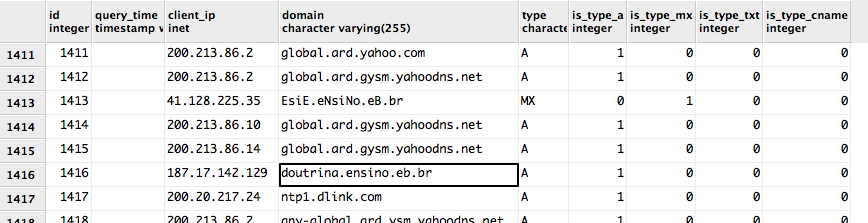
\includegraphics[width=\textwidth]{dns_queries}
\caption[Exemplos de entradas na tabela \textit{dns\_queries}]{Exemplos de entradas na tabela \textit{dns\_queries}} \label{fig:dns_queries}
\end{figure}

A tabela \textit{domains} contém informações referentes à cada domínio consultado. A coluna \textit{length} representa a quantidade de caracteres presentes no nome do domínio. A coluna \textit{numeric\_count} contém a informação de quantos caracteres numéricos estão presentes no domínio. A coluna \textit{readable\_string\_length} calcula a maior \textit{substring} legível do domínio, porém essa coluna não foi utilizada posteriormente, já que o ideal seria calcular o tamanho total legível da \textit{string}, mas devido a complexidade desse cálculo  ele não foi utilizado. A coluna \textit{is\_in\_whitelist} verifica se o domínio está na \textit{whitelist} utilizada, porém verificou-se que muitos domínios consultados conhecidos não estavam lá, abrindo margem para aprimoramento ao incrementar a \textit{whitelist} utilizada para o cenário do Exército Brasileiro. Finalmente, a coluna \textit{requisition\_degree} é bem interessante, informando o grau de requisição do domínio, ou seja, quantas máquinas diferentes também consultaram esse domínio. A Figura \ref{fig:domains} mostra exemplos de algumas entradas nessa tabela.

\begin{figure}
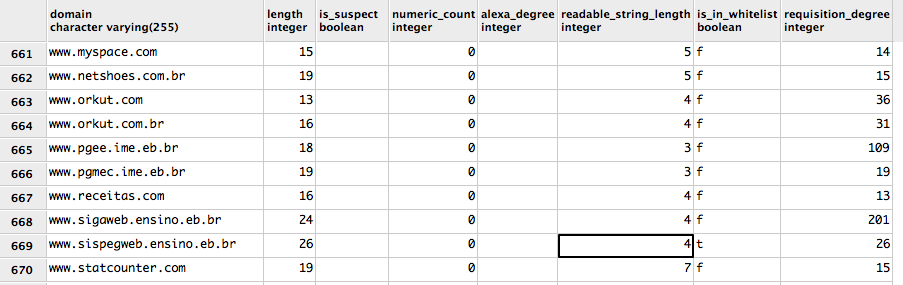
\includegraphics[width=\textwidth]{domains}
\caption[Exemplos de entradas na tabela \textit{domains}]{Exemplos de entradas na tabela \textit{domains}} \label{fig:domains}
\end{figure}

A tabela \textit{clients} representa as máquinas que fizeram requisições DNS no período de tempo analisado, sendo assim, ela é a mais importante para os algoritmos de aprendizado, já que o sistema está preocupado em descobrir as máquinas infectadas. O cálculo das colunas é feito com o auxílio das tabelas \textit{domains} e \textit{dns\_queries}, que guardam a informação de como o cliente tem se comportado na rede. Suas colunas foram motivadas pelas características que foram analisadas na seção \ref{sec:levantamento_das_caracteristicas}. Na figura \ref{fig:clients} são mostrados alguns valores para essas colunas. Devido ao elevado número de colunas nessa tabela, algumas delas foram omitidas para possibilitar a visualização.

\begin{figure}
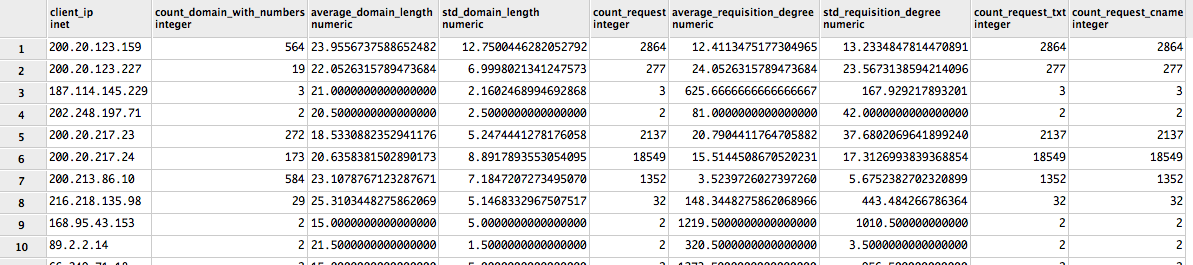
\includegraphics[width=\textwidth]{clients}
\caption[Exemplos de entradas na tabela \textit{clients}]{Exemplos de entradas na tabela \textit{clients}} \label{fig:clients}
\end{figure}

\section{Visão Geral do Sistema}
A aplicação desenvolvida serve para auxiliar na detecção de botnets. Esse auxílio é feito baseado em informações coletadas por um servidor de DNS. Para oferecer informações relevantes ao usuário, utilizando os algoritmos de agrupamento, a aplicação segue um fluxo básico, constituídos por etapas distintas: Leitura do Log DNS, Cálculo das Informações dos Domínios, Cálculo das Características das Máquinas, Seleção das Configurações, Execução do Algoritmo de Agrupamento e Disponibilização dos Resultados no Arquivo XLS. A Figura \ref{fig:program_flow} mostra um diagrama do fluxo básico de funcionamento do sistema.

\begin{figure}
\centering
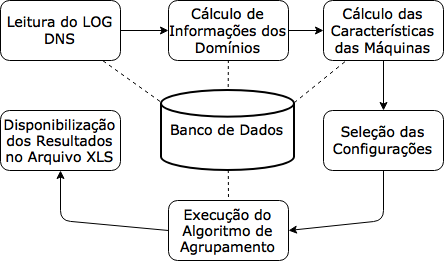
\includegraphics[width=12cm]{program_flow}
\caption[Diagram do Fluxo do Programa]{Diagrama do Fluxo do Programa} \label{fig:program_flow}
\end{figure}

As primeiras etapas que devem ser cumpridas, são as seguintes: Leitura de Log DNS, Cálculo das Informações das Informações dos Domínios e Cálculo das Características que são concluídas durante o caso de uso descrito na Tabela \ref{tab:use_case_load_file}. Na etapa de Leitura de Log DNS, é feita a extração das informações brutas coletadas pelo servidor DNS para o banco de dados. Nas etapas de Cálculo, as informações são calculadas utilizando chamadas as funções de agrupamento do SQL. A Figura \ref{fig:screen_file_loaded} mostra o estado da aplicação após a conclusão do caso de uso Carregar Arquivo de Log DNS, onde pode ser visto que a aplicação libera a utilização das opções ``Agrupar'' e ``Visualizar''.

\begin{figure}
\centering
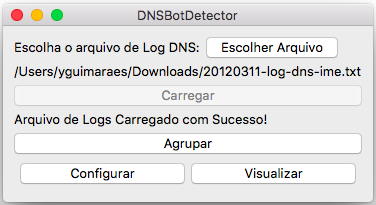
\includegraphics[width=10cm]{screen_file_loaded}
\caption[Tela do Sistema após Executar o Caso de Uso Carregar Arquivo de Log DNS]{Tela do Sistema após Executar o Caso de Uso Carregar Arquivo de Log DNS} \label{fig:screen_file_loaded}
\end{figure}

A Etapa de Seleção das Configurações, descrita pelo caso de uso na Tabela \ref{tab:use_case_config} é opcional, pois caso não seja realizada a aplicação carregará os valores padrão ou os utilizados em outro uso prévio da ferramenta. Essa etapa serve para que o usuário escolha as características que deseje que o algoritmo de agrupamento utilize, especifique o algoritmo de agrupamento desejado e o número de grupos que devem ser formados. A Figura \ref{fig:screen_config} mostra a tela na qual o usuário pode realizar essas configurações.

\begin{figure}
\centering
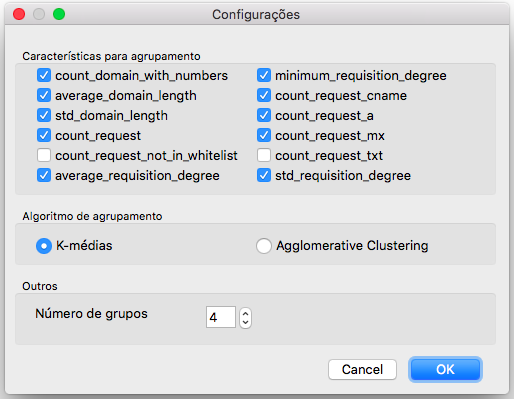
\includegraphics[width=10cm]{screen_config}
\caption[Tela do Sistema para Realizar a Seleção das Configurações]{Tela do Sistema para Realizar a Seleção das Configurações} \label{fig:screen_config}
\end{figure}

Por fim, as etapas de Execução do Algoritmo de Agrupamento e Disponibilização dos Resultados no Arquivo XLS acontecem na execução do caso de uso na Tabela \ref{tab:use_case_clustering}. Nessa etapa, o algoritmo de agrupamento escolhido é executado com os parâmetros selecionados na Etapa de Seleção das Configurações para as máquinas que estavam presentes no arquivo de log DNS utilizado. Em seguida, os resultados do algoritmo de agrupamento são persistidos no arquivo XLS com nome e caminho definidos pelo usuário da aplicação. Nesse arquivo, cada aba representa um grupo que foi identificado pelo algoritmo e contém as máquinas presentes nos respectivos grupos. A Figura \ref{fig:screen_xls_file} mostra a visualização desse arquivo.

\begin{figure}
\centering
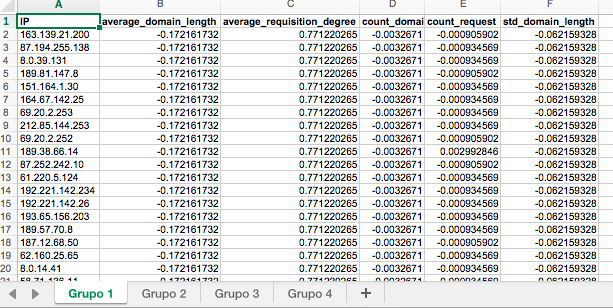
\includegraphics[width=13cm]{screen_xls_file}
\caption[\textit{Layout} do Arquivo XLS Gerado com os Resultados do Agrupamento]{\textit{Layout} do Arquivo XLS Gerado com os Resultados do Agrupamento} \label{fig:screen_xls_file}
\end{figure}

\begin{figure}
\centering
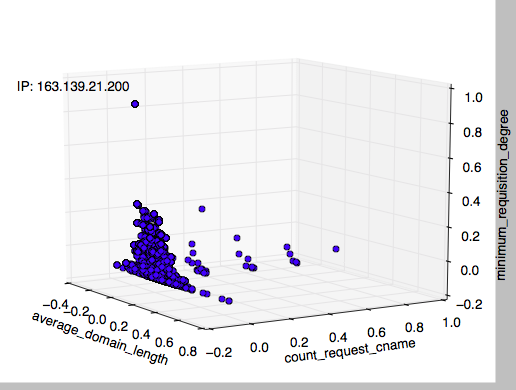
\includegraphics[width=12cm]{3d_graf_example}
\caption[\textit{Layout}  do Gráfico Gerado com um Ponto Isolado Selecionado]{\textit{Layout}  do Gráfico Gerado com um Ponto Isolado Selecionado} \label{fig:3d_graf_example}
\end{figure}

A aplicação apresenta também a funcionalidade de geração de gráficos. Uma funcionalidade da aplicação se encontra fora do fluxo principal da técnica de inteligência artificial, mas se mostrou preciosa para auxiliar na seleção das melhores características, além de permitir encontrar máquinas suspeitas visualmente. Os casos de uso dessa parte se encontram descritos nas tabelas \ref{tab:use_case_visualize} e \ref{tab:use_case_identify}.

Esses gráficos permitem identificar como as máquinas estão distribuídas espacialmente de acordo com as características selecionadas. Ou seja, o usuário pode selecionar 2 ou 3 características e visualizar o gráfico de como elas se encontram distribuídas no espaço. Isso permite identificar se as características utilizadas são úteis, ao exibir como a distribuição das máquinas se comporta com os valores de características selecionadas. Além disso, o usuário pode identificar os endereços de IP dos pontos que estão muito fora da normalidade, como na Figura \ref{fig:3d_graf_example} comportamento que pode ser considerado suspeito, auxiliando na detecção mais uma vez.
